\documentclass[aspectratio=169,xcolor=dvipsnames]{beamer}
\usepackage[normalem]{ulem}
\usepackage{comp2402}
\title{Abstract Data Types/Interfaces}
\author{Pat Morin \\ COMP2402}
\date{}

\begin{document}

\begin{frame}
  \titlepage
\end{frame}

\begin{frame}
  \frametitle{Abstract Data Types}
 
  \note{An abstract data type is also called an interface in many programming languages.} 
  \begin{itemize}
   \item<+->Describes what a data structure \emph{does}:
     \begin{itemize}
        \item<+->supported operations (the \emph{interface})
         \note{It describes the operations a data structure supports, this is also sometimes called the interface}
        \item<+->meaning of operations (the \emph{semantics})
         \note{It also describes what those operations mean, this is sometimes called the semantics.}
     \end{itemize}
   %\item<+-> Sometimes called the \emph{interface}
   \item<+-> \sout{Representation and implementation}
     \note{An abstract data type \emph{does not} describe how the data structure is represented or how it is implemented.
       An abstract data type answers the question: ``What does it do?'' It doesn't answer the question ``How does it do it?''
}
  \end{itemize}
\end{frame}

\begin{frame}
  \frametitle{Abstract Data Types/Interfaces}

  \begin{center}
   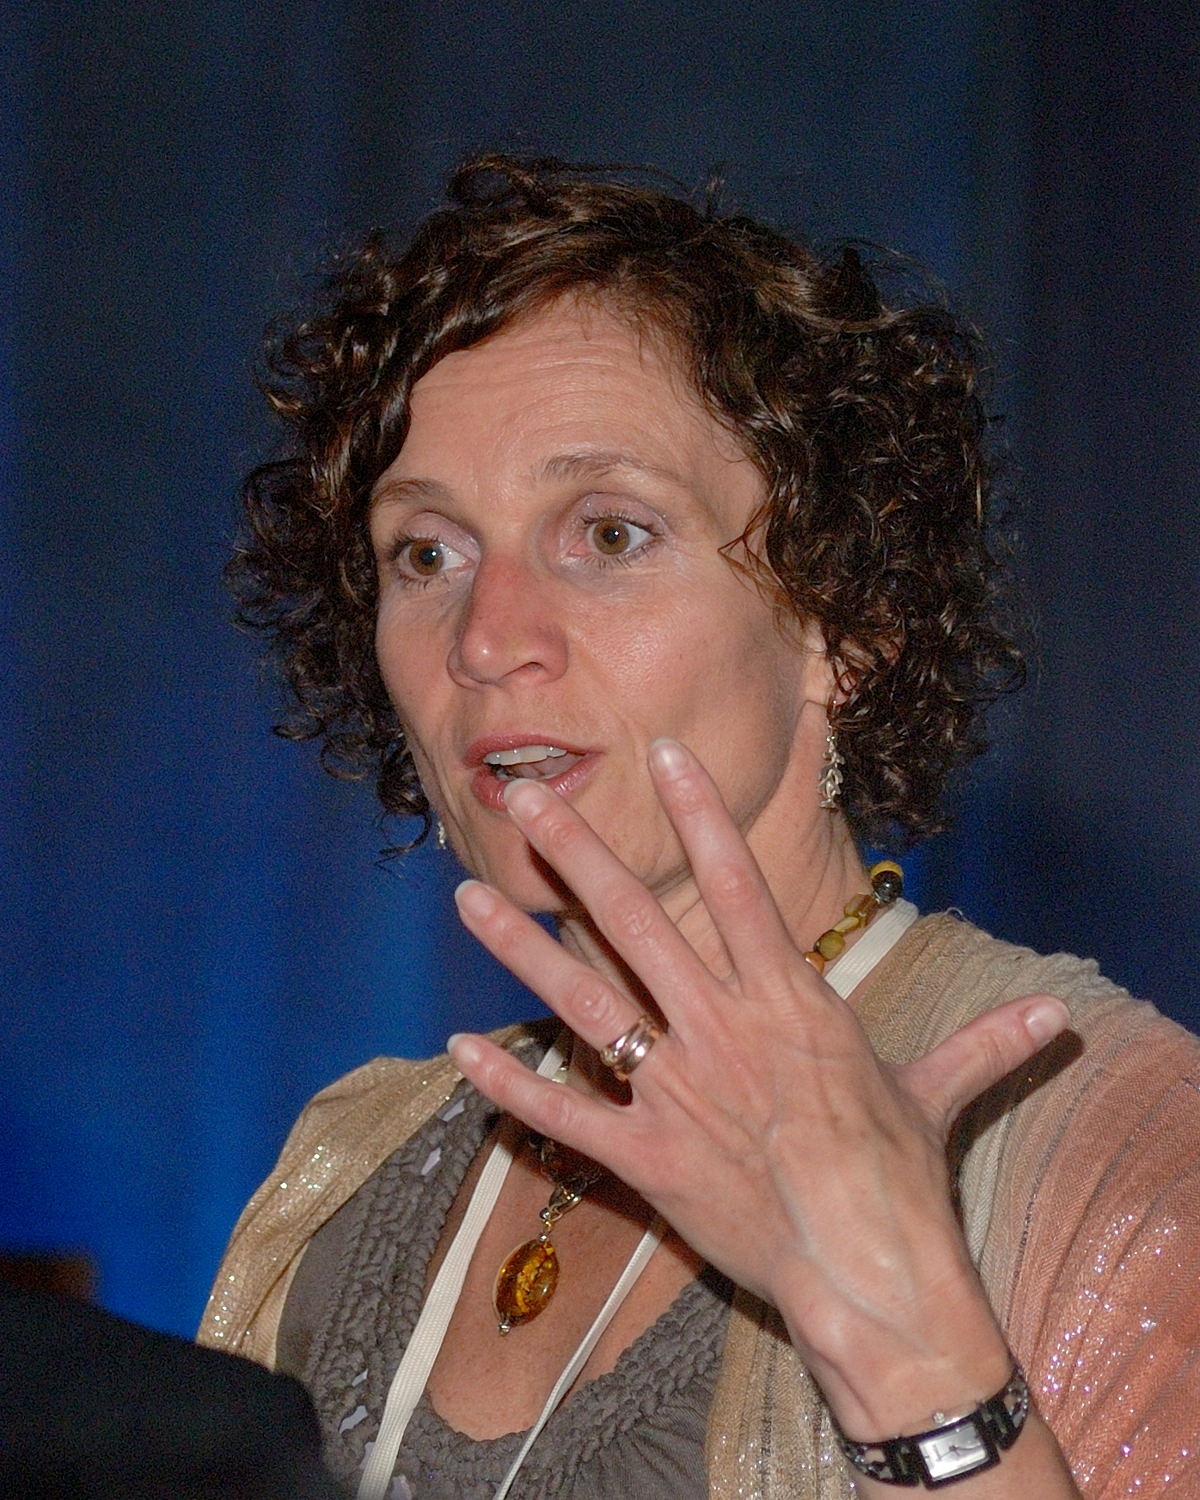
\includegraphics[height=.65\textheight]{images/liskov}\\
   B.~Liskov at the Turing Centenary Celebration (Wikimedia commons)
  \end{center}
  \note{The idea of abstracting a data structure's operations away from 
        it's implementation was introduced in a 1974 paper by 
        2008 ACM Turing Award Winner Barbara Liskov along with 
        coauthor Stephen N. Zilles.

        Rather than try for a formal definition, we'll jump in and 
        describe some of the abstract data types studied in this course.}
\end{frame}

\begin{frame}
  \frametitle{The List Interface}
 
  \begin{itemize}
    \item<+-> Represents a \emph{sequence} of $n$ items\newline
     \begin{center}
      \only<1>{\includegraphics{figs/list-interface-1}}%
      \only<2>{\includegraphics{figs/list-interface-2}}%
      \only<3->{\includegraphics{figs/list-interface-3}}%
     \end{center}
    \item<+> Elements indexed by position, $0,\ldots,n-1$.
    \item<+-> Operations: \only<+->{#size()#}%
                        \only<+->{, #get(i)#}%
                        \only<+->{, #set(i,x)#}%
                        \only<+->{, #add(i,x)#}%
                        \only<+->{, #remove(x)#}
  \end{itemize}
\end{frame}




\end{document}

